\section{Larger runtime costs for Compressed Sensing Reconstructions}\label{hypo}
The MeerKAT instrument produces a new magnitude of data volume. An image with several million pixels gets reconstructed from billions of Visibility measurements. Although MeerKAT measures a large set of Visibilities, the measurements are still incomplete. We do not have all the information available to reconstruct an image. Essentially, this introduces "fake" structures in the image, which a reconstruction algorithm has to remove. Additionally, the measurements are noisy.

We require an image reconstruction algorithm which removes the "fake" structures from the image, and removes the noise from the measurements. The large data volume of MeerKAT requires the algorithm to be both scalable and distributable. Over the years, several reconstruction algorithms were developed, which can be separated into two classes: Algorithms based on CLEAN, which are cheaper to compute and algorithms based on Compressed Sensing, which create higher quality reconstructions.

CLEAN based algorithms represent the reconstruction problem as a deconvolution. First, they calculate the "dirty" image, which is corrupted by noise and fake image structures. The incomplete measurements essentially convolve the image with a Point Spread Function ($PSF$). CLEAN estimates the $PSF$ and searches for a deconvolved version of the dirty image. In each CLEAN iteration, it searches for the highest pixel in the dirty image, subtracts a fraction $PSF$ at the location. It adds the fraction to the same pixel location of a the "cleaned" image. After several iterations, the cleaned image contains the deconvolved version of the dirty image. CLEAN accounts for noise by stopping early. It stops when the highest pixel value is smaller than a certain threshold. This results in a light-weight and robust reconstruction algorithm. CLEAN is comparatively cheap to compute, but does not produce the best reconstructions and is difficult to distribute on a large scale.

Compressed Sensing based algorithms represent the reconstruction as an optimization problem. They search for the optimal image which is as close to the Visibility measurements as possible, but also has the smallest regularization penalty. The regularization encodes our prior knowledge about the image. Image structures which were likely measured by the instrument result in a low regularization penalty. Image structures which were likely introduced by noise or the measurement instrument itself result in high penalty. Compressed Sensing based algorithms explicitly handle noise and create higher quality reconstructions than CLEAN. State-of-the-art Compressed Sensing algorithms show potential for distributed computing. However, they currently do not scale on MeerKATs data volume. They require too many computing resources compared to CLEAN based algorithms.
 
This project searches for a way to reduce the runtime costs of Compressed Sensing based algorithms. One reason for the higher costs is due to the non-uniform FFT Cycle. State-of-the-art CLEAN and Compressed Sensing based algorithms both use the non-uniform FFT approximation in a cycle during reconstruction. The interferometer measures the Visibilities in a continuous space in a non-uniform pattern. The image is divided in a regularly spaced, discrete pixels. The non-uniform FFT creates an approximate, uniformly sampled image from the non-uniform measurements. Both, CLEAN and Compressed Sensing based algorithms use the non-uniform FFT to cycle between non-uniform Visibilities and uniform image. However, a Compressed Sensing algorithm requires more non-uniform FFT cycles for reconstruction. 

CLEAN and Compressed Sensing based algorithms use the non-uniform FFT in a similar manner. However, there are slight differences in the architecture. This project hypothesises that 
The previous project searched for an alternative to the non-uniform FFT cycle. Although there are alternatives, there is currently no replacement which leads to lower runtime costs for Compressed Sensing. Current research is focused on reducing the number of non-uniform FFT cycles for Compressed Sensing algorithms.

CLEAN based algorithms use the Major Cycle Architecture for reconstruction. Compressed Sensing based algorithms use a similar architecture, but with slight modifications. Our hypothesis is that we may reduce the number of non-uniform FFT cycles for Compressed Sensing by using CLEAN's Major Cycle Architecture.

\subsection{CLEAN: The Major Cycle Architecture}

\begin{figure}[h]
	\centering
	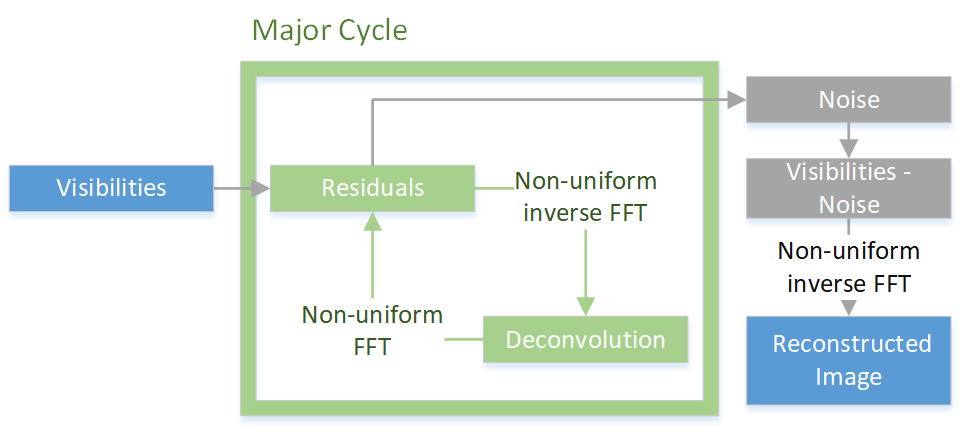
\includegraphics[width=0.80\linewidth]{./chapters/02.hypo/Major-Minor.png}
	\caption{The Major Cycle Architecture}
	\label{hypo:major}
\end{figure}

Figure \ref{hypo:major} depicts the Major Cycle Architecture used by CLEAN algorithms. First, the Visibilities get transformed into an image with the non-uniform FFT. The resulting dirty image contains the corruptions of the measurement instrument and noise. A deconvolution algorithm, typically CLEAN, removes the corruption of the instrument with a deconvolution. When the deconvolution stops, it should have removed most of the observed structures from the dirty image. The rest, mostly noisy part of the dirty image gets transformed back into residual Visibilities and the cycle starts over.

In the Major Cycle Architecture, we need several deconvolution attempts before it has distinguished the noise from the measurements. Both the non-uniform FFT and the deconvolution are approximations. By using the non-uniform FFT in a cycle, it can reconstruct an image at a higher quality. For MeerKAT reconstruction with CLEAN, we need approximately 4-6 non-uniform FFT cycles for a reconstruction.


\subsection{Compressed Sensing Architecture}\label{hypo:CSArch}

\begin{figure}[h]
	\centering
	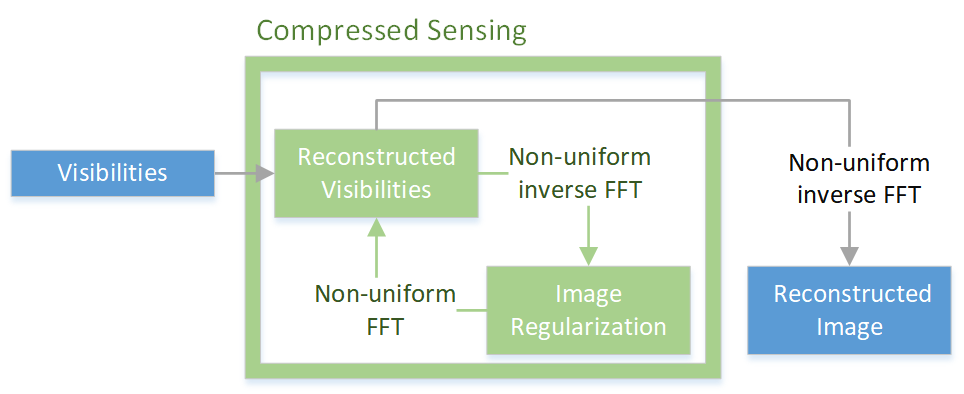
\includegraphics[width=0.80\linewidth]{./chapters/02.hypo/CS.png}
	\caption{State-of-the-art Compressed Sensing Reconstruction Architecture}
	\label{hypo:cs}
\end{figure}

Figure \ref{hypo:cs} depicts the architecture used by Compressed Sensing reconstructions. The Visibilities get transformed into an image with the non-uniform FFT approximation. The algorithm then modifies the image so it reduces the regularization penalty. The modified image gets transformed back to Visibilities and the algorithm then minimizes the difference between measured and reconstructed Visibilities. This is repeated until the algorithm converges to an optimum.

In this architecture, state-of-the-art Compressed Sensing algorithms need approximately 10 or more non-uniform FFT cycles to converge. It is one source for the higher runtime costs. For MeerKAT reconstructions the non-uniform FFT tends to dominate the runtime costs. A CLEAN reconstruction with the Major Cycle Architecture already spends a large part of its time in the non-uniform FFT. Compressed Sensing algorithms need even more non-uniform FFT cycle on top of the "Image Regularization" step being generally more expensive than CLEAN deconvolution. There is one upside in this architecture: State-of-the-art algorithms managed to distribute the "Image Regularization" operation.

\subsection{Hypothesis for reducing costs of Compressed Sensing Algorithms}
Compressed Sensing Algorithms are not bound to the Architecture presented in section \ref{hypo:CSArch}. For example, we can design a Compressed Sensing based deconvolution algorithm and use the Major Cycle Architecture instead. 

Our hypothesis is: We can create a Compressed Sensing based deconvolution algorithm which is both distributable and creates higher quality reconstructions than CLEAN. Because it also uses the Major Cycle architecture, we reckon that the Compressed Sensing deconvolution requires a comparable number of non-uniform FFT cycles to CLEAN. This would result in a Compressed Sensing based reconstruction algorithm with similar runtime costs to CLEAN, but higher reconstruction quality and higher potential for distributed computing.


